\begin{tikzpicture}
	\pgfplotsset{/tikz/font={\small}}
	\begin{axis}[
		grid=both,
		width=0.95\textwidth,
		height=0.95\textheight,
		x tick label style={
		/pgf/number format/1000 sep=},
		% scaled y ticks = false,
		% y tick label style={
		% 	/pgf/number format/.cd,
		% 	fixed,
		% 	set thousands separator={\thinspace},
		% 	fixed zerofill,
		% 	precision=0,
		% },
		ymax=100, ymin=0,
		ytick={0,20,...,100},
		ylabel={PB per month},
		enlarge y limits=false,
		enlarge x limits=0.04,
		legend pos=north west,
		legend cell align=left,
		ybar interval,
		xtick=data,
		xtick align=inside,
		]

		\addlegendentry{Internet video}
		\addplot coordinates {
		(2014, 21.624)
		(2015, 27.466)
		(2016, 36.456)
		(2017, 49.068)
		(2018, 66.179)
		(2019, 89.319)
		(2020, 0) % this line needs to be added so that it plots the previous one
		};

		\addlegendentry{Web, email, and data}
		\addplot coordinates {
		(2014,  5.853)
		(2015,  7.694)
		(2016,  9.476)
		(2017, 11.707)
		(2018, 14.002)
		(2019, 16.092)
		(2020, 0) % this line needs to be added so that it plots the previous one
		};

		\addlegendentry{File sharing}
		\addplot coordinates {
		(2014, 6.090)
		(2015, 6.146)
		(2016, 6.130)
		(2017, 6.168)
		(2018, 6.231)
		(2019, 6.038)
		(2020, 0) % this line needs to be added so that it plots the previous one
		};

		\addlegendentry{Online gaming}
		\addplot coordinates {
		(2014, 0.027)
		(2015, 0.033)
		(2016, 0.048)
		(2017, 0.078)
		(2018, 0.109)
		(2019, 0.143)
		(2020, 0) % this line needs to be added so that it plots the previous one
		};
	\end{axis}
\end{tikzpicture}
